%-------------------------------------------------------------------------------
% yum_padsynth
%-------------------------------------------------------------------------------
%
% \file        yum_padsynth.tex
% \library     Documents
% \author      Chris Ahlstrom
% \date        2015-06-07
% \update      2016-02-28
% \version     $Revision$
% \license     $XPC_GPL_LICENSE$
%
%     Provides the PADsynth section of yoshimi-user-manual.tex.
%
%-------------------------------------------------------------------------------

\section{PADsynth}
\label{sec:padsynth}

   The \textsl{Yoshimi} PADsynth dialog is a complex dialog for creating a
   pad instrument,  "PADsynth" or "PADnote" is engine that makes very
   beautiful pads and other instruments. (These instruments can be exported
   for use with other programs too).

   The PADsynth dialog consists of two major tabs, "Harmonic Structure" and
   "EnvelopesLFOs".  Each of these tabs is fairly complex, so the discussion
   will break the tabs down by sub-sections.

\subsection{PADsynth / Algorithm}
\label{subsec:padsynth_algorithm}

\subsubsection{PADsynth / Algorithm / General}
\label{subsubsec:padsynth_algorithm_general}

   This algorithm generates very beautiful sounds, even if its idea is much
   simpler than other algorithms. It generates a perfectly looped wave-table
   sample which can be used in instruments. It easily generates sounds of
   ensembles, choirs, metallic sounds (bells) and many other types of sound.
   Paul Nasca wanted to make this algorithm known, and everyone is welcome to
   learn and use this algorithm into one's projects or products (non-commercial
   or commercial).
   
   Quote \cite{zyndoc}:

   \begin{quotation}
      You will not be disappointed by this algorithm.

      I hope that this algorithm will be implemented in many software/hardware
      synthesizers. Use it, spread it, write about it, create beautiful
      instruments with it. If your synthesizer uses plenty of samples, you can
      use this algorithm to generate many ready-to-use samples.

      This algorithm, this page, the images, the implementations from this
      page, the audio examples, the parameter files from this page
      are released under Public Domain by Nasca Octavian Paul.
      e-mail: zynaddsubfx AT yahoo DOT com
   \end{quotation}

   In order to understand how this algorithm works, one needs to be familiar
   with how to think about musical instruments. Please read an introduction
   for the description of the meaning and the importance of bandwidth of each
   harmonic and randomness.

   This algorithm generates some large wave-tables that can be played at
   different speeds to get the desired sound. This algorithm describes only
   how these wave-tables are generated. The result is a perfectly looped
   wave-table.  Unlike other synthesis methods, which use the
   Inverse Fast Fourier Transform, this one does not use overlap/add methods
   and there is only one IFFT for the whole sample.

   The basic steps are:

   \begin{enumber}
      \item Make a very large array that represents the amplitude spectrum of
         the sound (all default values are zero).
      \item Generate the distribution of each harmonic in the frequency
         spectrum and add it to the array.
      \item Put random phases to each frequency of the spectrum.
      \item Do a single Inverse Fourier Transform of the whole spectrum. There
         is no need of any overlapping windows, because there is only one
         single IFFT for the whole sample. 
   \end{enumber}

   The output is a sample which can be used as a wave-table In the next image,
   the steps are represented graphically:

      TODO:  A GRAPHIC

\subsubsection{PADsynth / Algorithm / Harmonic Bandwidth}
\label{subsubsec:padsynth_algorithm_harmonic_bandwidth}

   We consider one harmonic (overtone) as being composed of many frequencies.
   These sine components of one harmonic are spread over a certain band of
   frequencies.  Higher harmonics have a wider bandwidth. In natural
   choirs/ensembles the bandwidth is proportional to the frequency of the
   harmonic.
   
   Here is an example of a spectrum of an instrument generated by ZynAddSubFX:

      TODO:  A GRAPHIC, full spectrum, closeup of the spectrum

   The harmonics becomes wider and wider, until a certain frequency, where
   they may merge into a noise band (as in the full spectrum image from above
   shows). This is a normal thing and we recommend to not avoid this by
   limiting the bandwidth of the harmonics.

   The frequency distribution of one harmonic/overtone (or the harmonic
   profile).

   This describes the function of the spread of the harmonic.
   Here are some examples of how they can be spread:

   a) A special case is where there is only a single sine component inside the
   harmonic In this case, the harmonic and the "sine component" are the same
   thing.

   b) Detuned. In this case there are two sine components which are detuned.

   c) Evenly spread inside the harmonic (all components has the same amplitude)

   d) Normal (Gaussian) distribution. The sine components amplitude are bell
   shaped. The largest amplitude is in the center of the band. This distribution
   gives the most natural sounds (it simulates a very, very large ensemble).

   Of course, one can use many other profiles of the harmonic. ZynAddSubFX's
   PADsynth module offers many ways to generate the harmonic profile.  Also, it's
   very important that the harmonic must have the same amplitude, regardless of
   the profile functions/parameters and the bandwidth.

   For many more details of this algorithm, see Paul Nasca's document
   \cite{zyndoc}.

\paragraph{Tip: Using the PADsynth}
\label{tips_using_the_padsynth}
\index{tips!padsynth usage}

   Keep in mind that the resulting wave-tables are perfectly looped.
   When using the wave-tables for instruments, on each NoteOn, start from a
   random position and not from the start. This avoids hearing the same sound
   on each keystroke.

   One can use the same wave-table for generating stereo sounds, by playing
   the same wave-table at different positions for left and right. The best is
   to create a difference between left right of N/2.

   Generate different wave-tables for different pitches and use the one that
   is closest to the desired pitch.

   Upsample or downsample the amplitude array of the harmonic before running
   the algorithm, according to the fundamental frequency. In this case we need
   to set a parameter "base\_frequency" which represents the frequency where
   the array is left unchanged. 

   Example:
   We have A\_orig[]={1,2,1,3,0,0,1,0} and base\_frequency is equal to 440 Hz
   Here are some cases:

A[] for 440 Hz: is the same as A\_orig[] 

A[] for 220 Hz: is the A\_orig[] upsampled by factor of 2

so: A[]={1, 1, 1.5, 2, 1.5, 1, 2, 3, 1.5, 0, 0, 0, 0.5, 1, 0.5, 0}

(the original A\_orig amplitudes are shown as bold) 

A[] for 880 Hz: the A\_orig[] is downsampled by a factor of 2

so: A[]={1.5, 2, 0, 0.5} 

A[] for F Hz: the A\_orig[] is scaled by a factor of 440/F.

   Even if this idea is very simple, the resulting sounds are very natural,
   because it keeps the spectrum constant according to the frequency of the
   harmonic and not to the number of the harmonic. This follows the point 4
   from the document where I described some principles regarding synthesis.

\subsection{PADsynth / Harmonic Structure}
\label{subsec:padsynth_harmonic_structure}

\begin{figure}[H]
   \centering 
   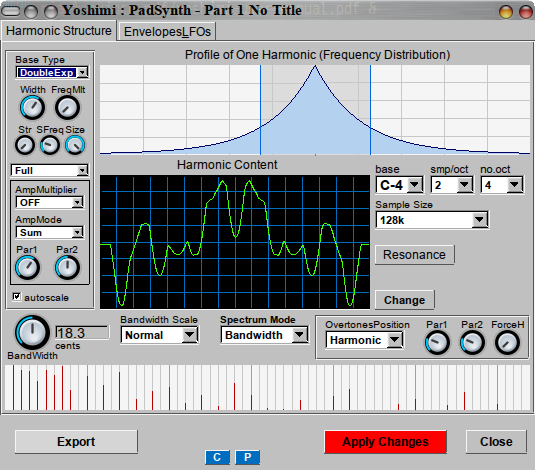
\includegraphics[scale=1.0]{bottom-panel/instrument-edit/PAD/PADsynth-parameters-harmonic-structure.jpg}
   \caption{PADsynth Edit Dialog}
   \label{fig:padsynth_edit_dialog}
\end{figure}

   \begin{enumber}
      \item \textbf{Basics} (section)
      \item \textbf{Harmonic} (section)
      \item \textbf{Resonance} (section)
      \item \textbf{Change} (section)
      \item \textbf{Bandwidth and Position} (section)
      \item \textbf{Export} (section)
      \item \textbf{C}
      \item \textbf{P}
      \item \textbf{Apply Changes}
      \item \textbf{Close}
   \end{enumber}

\subsubsection{PADsynth / Harmonic Structure / Basics}
\label{subsubsec:padsynth_harmonic_structure_basics}

   \begin{enumber}
      \item \textbf{BaseType}
      \item \textbf{Width}
      \item \textbf{FreqMlt}
      \item \textbf{Str}
      \item \textbf{SFreq}
      \item \textbf{Size}
      \item \textbf{Full/Upper/Lower}
      \item \textbf{AmpMultiplier}
      \item \textbf{AmpMode}
      \item \textbf{Par1}
      \item \textbf{Par2}
   \end{enumber}

   \setcounter{ItemCounter}{0}      % Reset the ItemCounter for this list.

   \itempar{BaseType}{padsynth!harmonic type}
   Base Type of Harmonic.

\begin{figure}[H]
   \centering 
   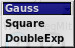
\includegraphics[scale=1.0]{bottom-panel/instrument-edit/PAD/base-type.jpg}
   \caption{Base Type of Harmonic}
   \label{fig:padsynth_base_type_of_harmonic}
\end{figure}

   Values: \texttt{Gauss*, Square, DoubleExp}

   \itempar{Width}{padsynth!harmonic width}
   Width of Harmonic.

   Values: \texttt{1 to 127?}

   \itempar{FreqMlt}{padsynth!freq mult}
   Frequency Multiplier.

   Values: \texttt{1 to 127?}

   \itempar{Str}{padsynth!harmonic stretch}
   Stretch.

   \itempar{SFreq}{padsynth!harmonic sfreq}
   Harmonic Sfreq?

   \itempar{Size}{padsynth!harmonic size}
   Harmonic Size.

   \itempar{Full/Upper/Lower}{padsynth!harmonic fup}
   Harmonic Spread???

\begin{figure}[H]
   \centering 
   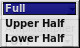
\includegraphics[scale=1.0]{bottom-panel/instrument-edit/PAD/full-upper-lower.jpg}
   \caption{PADsynth Full/Upper/Lower Harmonics}
   \label{fig:padsynth_full_upper_lower}
\end{figure}

   Values: \texttt{Full*, Upper Half, Lower Half}

   \itempar{AmpMultiplier}{padsynth!amp mult}
   Amplitude Multiplier.

\begin{figure}[H]
   \centering 
   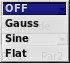
\includegraphics[scale=1.0]{bottom-panel/instrument-edit/PAD/amp-multiplier.jpg}
   \caption{PADsynth Amplitude Multiplier}
   \label{fig:padsynth_amplitude_multiplier}
\end{figure}

   Values: \texttt{OFF*, Gauss, Sine, Flat}

   \itempar{AmpMode}{padsynth!amp mode}
   Amplitude Mode.

\begin{figure}[H]
   \centering 
   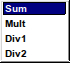
\includegraphics[scale=1.0]{bottom-panel/instrument-edit/PAD/amp-mode.jpg}
   \caption{PADsynth Amplitude Mode}
   \label{fig:padsynth_amplitude_mode}
\end{figure}

   Values: \texttt{Sum*, Mult, Div1, Div2}

   \itempar{Par1}{padsynth!harmonic par1}
   Harmonic Parameter 1?

   Values: \texttt{0 to 127?}

   \itempar{Par2}{padsynth!harmonic par2}
   Harmonic Parameter 2?

   Values: \texttt{0 to 127?}

\subsubsection{PADsynth / Harmonic Structure / Harmonic}
\label{subsubsec:padsynth_harmonic_structure_harmonic}

   \begin{enumber}
      \item \textbf{Profile of One Harmonic}
      \item \textbf{Harmonic Content Window}
      \item \textbf{base}
      \item \textbf{smp/oct}
      \item \textbf{no.oct}
      \item \textbf{Sample Size}
      \item \textbf{Resonance} (section)
      \item \textbf{Change} (section)
   \end{enumber}

   \setcounter{ItemCounter}{0}      % Reset the ItemCounter for this list.

   \itempar{Profile of One Harmonic}{padsynth!harmonic profile}
   Profile of One Harmonic (Frequency Distribution).

   \itempar{Harmonic Content Window}{padsynth!harmonic content}
   Harmonic Content Window.

   \itempar{base}{padsynth!harmonic base}

\begin{figure}[H]
   \centering 
   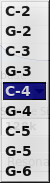
\includegraphics[scale=1.0]{bottom-panel/instrument-edit/PAD/base.jpg}
   \caption{Harmonic Base Dropdown}
   \label{fig:padsynth_harmonic_base_dropdown}
\end{figure}

   Values: \texttt{C-2, G-2, C-3, G-3, C-4*, G-4, C-5, G-5, G-6}

   \itempar{smp/oct}{padsynth!harmonic samples per oct}
   Harmonic Samples Per Octave?

\begin{figure}[H]
   \centering 
   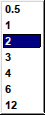
\includegraphics[scale=1.0]{bottom-panel/instrument-edit/PAD/smp-per-octave.jpg}
   \caption{Harmonic Samples Per Octave}
   \label{fig:padsynth_harmonic_samples_per_octave}
\end{figure}

   \itempar{no.oct}{padsynth!harmonic no. of octaves}
   Number of Octaves of Harmonic.

\begin{figure}[H]
   \centering 
   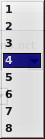
\includegraphics[scale=1.0]{bottom-panel/instrument-edit/PAD/number-of-octaves.jpg}
   \caption{Harmonic Number of Octaves}
   \label{fig:padsynth_harmonic_number_of_octaves}
\end{figure}

   Values: \texttt{1, 2, 3, 4*, 5, 6, 7, 8}

   \itempar{Sample Size}{padsynth!harmonic sample size}
   Harmonic Sample Size.

\begin{figure}[H]
   \centering 
   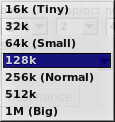
\includegraphics[scale=1.0]{bottom-panel/instrument-edit/PAD/sample-size.jpg}
   \caption{Harmonic Sample Size Dropdown}
   \label{fig:padsynth_harmonic_sample_size_dropdown}
\end{figure}

   Values: \texttt{16k (Tiny), 32k, 64k (Small), 128k*, 256k (Normal), 512k, 1M (Big)}

\subsubsection{PADsynth / Harmonic Structure / Bandwidth and Position}
\label{subsubsec:padsynth_harmonic_structure_bw_and_pos}

   \begin{enumber}
      \item \textbf{BandWidth}
      \item \textbf{cents}
      \item \textbf{Bandwidth Scale}
      \item \textbf{Spectrum Mode}
      \item \textbf{OvertonesPosition}
      \item \textbf{Par1}
      \item \textbf{Par2}
      \item \textbf{ForceH}
      \item \textbf{Harmonics Plot}
   \end{enumber}

   \setcounter{ItemCounter}{0}      % Reset the ItemCounter for this list.

   \itempar{BandWidth}{padsynth!bandwidth}
   Harmonics Bandwidth.

   Values: \texttt{0 to 127?}

   \itempar{cents}{padsynth!bandwidth reading}
   Bandwidth Reading (cents).

   \itempar{Bandwidth Scale}{padsynth!bandwidth scale}
   Bandwidth Scale.

\begin{figure}[H]
   \centering 
   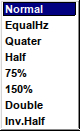
\includegraphics[scale=1.0]{bottom-panel/instrument-edit/PAD/bandwidth-scale.jpg}
   \caption{Harmonics Bandwidth Scale.}
   \label{fig:padsynth_harmonics_bandwidth_scale}
\end{figure}

   Values: \texttt{Normal, EqualHz, Quater, Half, 75\%, 150\%, Double, Inv.  Half}

   \itempar{Spectrum Mode}{padsynth!spectrum mode}
   Harmonics Spectrum Mode.

\begin{figure}[H]
   \centering 
   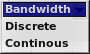
\includegraphics[scale=1.0]{bottom-panel/instrument-edit/PAD/spectrum-mode.jpg}
   \caption{PADsynth Harmonics Spectrum Mode}
   \label{fig:padsynth_harmonics_spectrum mode}
\end{figure}

   Values: \texttt{Bandwidth*, Discrete, Continuous}

   \itempar{OvertonesPosition}{padsynth!overtones}
   Overtones Position.

\begin{figure}[H]
   \centering 
   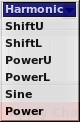
\includegraphics[scale=1.0]{bottom-panel/instrument-edit/PAD/overtones-position.jpg}
   \caption{PADsynth Overtones Position}
   \label{fig:padsynth_overtones_position}
\end{figure}

   Values: \texttt{Harmonic*, ShiftU, ShiftL, PowerU, PowerL, Sine, Power}

   \itempar{Par1}{padsynth!par1}
   PADSynth Bandwidth Parameters 1?

   \itempar{Par2}{padsynth!par2}
   PADSynth Bandwidth Parameters 2?

   \itempar{ForceH}{padsynth!forceh}
   PADSynth Bandwidth ForceH.

   \itempar{Harmonics Plot}{padsynth!harmonics plot}
   PADSynth Harmonics Plot.

\subsubsection{PADsynth / Harmonic Structure / Export}
\label{subsubsec:padsynth_harmonic_structure_export}

\begin{figure}[H]
   \centering 
   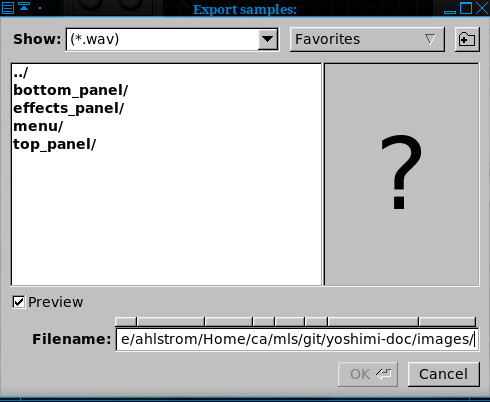
\includegraphics[scale=0.75]{bottom-panel/instrument-edit/PAD/export-dialog.jpg}
   \caption{Harmonics Structure Export Dialog}
   \label{fig:harmonics_structure_export_dialog}
\end{figure}

   This export dialog is a file dialog similar to other file dialogs
   in \textsl{Yoshimi}.

\subsubsection{PADsynth / Harmonic Structure / Resonance}
\label{subsubsec:padsynth_harmonic_structure_resonance}

   The PADsynth Harmonics resonance dialog is identical to the resonance
   dialog described in
   \sectionref{subsec:addsynth_resonance},
   except that it shows something that the ADDsynth version doesn't... an
   "Apply" button.

\subsubsection{PADsynth / Harmonic Structure / Change}
\label{subsubsec:padsynth_harmonic_structure_change}

   Harmonic Content Editor.  Another complex dialog.
   Like
   \figureref{fig:addsynth_oscillator_editor},
   it allows one to create an unlimited
   number of oscillators. 

\begin{figure}[H]
   \centering 
   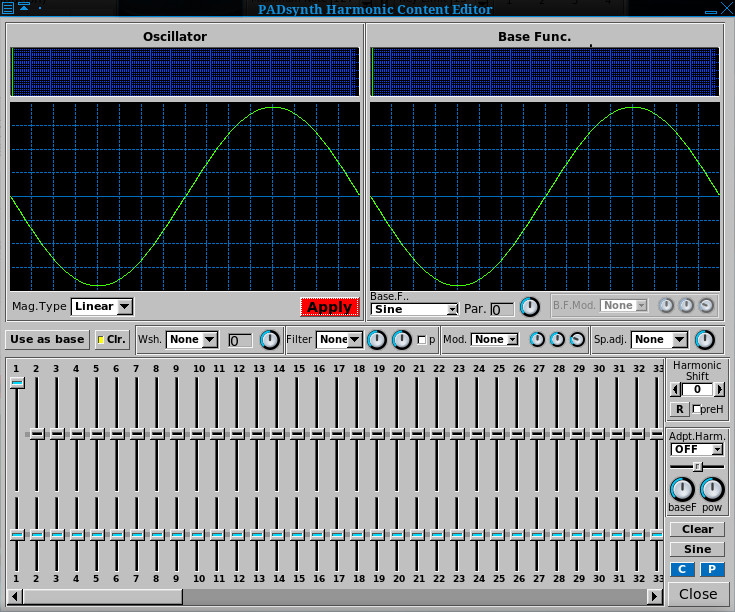
\includegraphics[scale=0.75]{bottom-panel/instrument-edit/PAD/harmonic-content-editor.jpg}
   \caption{Harmonic Content Editor}
   \label{fig:padsynth_harmonic_content_editor}
\end{figure}

   This dialog is complex enough that it makes sense to break it down into
   sub-sections.

   \begin{enumber}
      \item \textbf{Oscillator} (section)
      \item \textbf{Base Function} (section)
      \item \textbf{Middle} (section)
      \item \textbf{Harmonic} (section)
   \end{enumber}

\paragraph{PADsynth / Harmonic Structure / Change / Oscillator}
\label{paragraph:padsynth_harmonic_structure_change_oscillator}

   \begin{enumber}
      \item \textbf{Oscillator Spectrum Graph}
      \item \textbf{Oscillator Waveform Graph}
      \item \textbf{Mag.Type}
      \item \textbf{rnd} (ADDsynth Oscillator Editor only)
      \item \textbf{H.rnd} (ADDsynth Oscillator Editor only)
      \item \textbf{H.rnd knob} (ADDsynth Oscillator Editor only)
      \item \textbf{Apply} (not present in ADDsynth Oscillator Editor)
   \end{enumber}

   TODO:  Describe the 3 ADDsynth elements noted above.

   rnd - Set the randomness of the oscillator output. There are 2 types of
   randomnesses, first is group randomness(the oscillator starts at random
   position), second is from -64(max) to -1 (min) and each harmonic
   (the oscillator is phase distorted) is from 1(min) to 63 (max). 0 is no
   randomness. One could use this parameter to make warm sounds like
   analogue synthesizers.

   \setcounter{ItemCounter}{0}      % Reset the ItemCounter for this list.

   \itempar{Oscillator Spectrum Graph}{padsynth!oscillator graph}
   Oscillator Spectrum Graph.

   \itempar{Oscillator Waveform Graph}{padsynth!waveform graph}
   Oscillator Waveform Graph.

   \itempar{Mag.Type}{padsynth!mag type}
   Oscillator Magnitude Type.
   Sets how the magnitudes from the user interface behave.  See the values
   below.

\begin{figure}[H]
   \centering 
   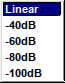
\includegraphics[scale=1.0]{bottom-panel/instrument-edit/PAD/harmonic-content-mag-type.jpg}
   \caption{PADsynth Harmonic Content Mag Type}
   \label{fig:padsynth_harmonic_content_mag_type}
\end{figure}

   Values: \texttt{Linear*, -40dB, -60db, -80dB, -100dB}

   \itempar{Apply}{padsynth!apply button}
   PADsynth Harmonic Content Editor Apply Button.

\paragraph{PADsynth / Harmonic Structure / Change / Base Function}
\label{paragraph:padsynth_harmonic_structure_change_base_function}

   \begin{enumber}
      \item \textbf{Base Func. Spectrum Graph}
      \item \textbf{Base Func. Waveform Graph}
      \item \textbf{Base F..}
      \item \textbf{Par. Value}
      \item \textbf{Par. Wheel}
      \item \textbf{B.F.Mod.}
      \item \textbf{Wheel 1}
      \item \textbf{Wheel 2}
      \item \textbf{Wheel 3}
   \end{enumber}

   \setcounter{ItemCounter}{0}      % Reset the ItemCounter for this list.

   \itempar{Base Func. Spectrum Graph}{padsynth!base function spectrum}
   Harmonic Base Function Spectrum Graph.

   \itempar{Base Func. Waveform Graph}{padsynth!base function waveform}
   Harmonic Base Function Waveform Graph.

   \itempar{Base F..}{padsynth!base function}
   Harmonic Base Function.
   Sets what function to use as the harmonics base function.
   One can use any base function as harmonics. 

\begin{figure}[H]
   \centering 
   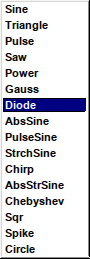
\includegraphics[scale=1.0]{bottom-panel/instrument-edit/PAD/harmonic-content-base-function.jpg}
   \caption{PADsynth Harmonic Content Base Function}
   \label{fig:padsynth_harmonic_content_base_function}
\end{figure}

   Values: \texttt{Sine*, Triangle, Pulse, Saw, Power, Gauss, Diode, AbsSine,
           PulseSine, StrchSine, Chirp, AbsStrSine, Chebyshev,
           Sqr, Spike, Circle}

   \itempar{Par. Value}{padsynth!par value}
   PADsynth Parameter Value.

   \itempar{Par. Wheel}{padsynth!par wheel}
   PADsynth Parameter Wheel.
   Change the parameter of the base function. 

   \itempar{B.F.Mod.}{padsynth!bf mod}
   PADSynth Base Frequency Mod.

   \itempar{Wheel 1}{padsynth!wheel 1}
   PADsynth Wheel 1.

   \itempar{Wheel 2}{padsynth!wheel 2}
   PADsynth Wheel 2.

   \itempar{Wheel 3}{padsynth!wheel 3}
   PADsynth Wheel 3.


\paragraph{PADsynth / Harmonic Structure / Change / Middle}
\label{paragraph:padsynth_harmonic_structure_change_middle}

   \begin{enumber}
      \item \textbf{Use as base}
      \item \textbf{Clr.}
      \item \textbf{Wsh.}
      \item \textbf{Wsh Value}
      \item \textbf{Wsh Wheel}
      \item \textbf{Filter}
      \item \textbf{Filter Wheel 1}
      \item \textbf{Filter Wheel 2}
      \item \textbf{Filter p}
      \item \textbf{Mod.}
      \item \textbf{Mod. Wheel 1}
      \item \textbf{Mod. Wheel 2}
      \item \textbf{Mod. Wheel 3}
      \item \textbf{Sp.adj.}
      \item \textbf{Sp.adj. Wheel}
   \end{enumber}

   \setcounter{ItemCounter}{0}      % Reset the ItemCounter for this list.

   \itempar{Use as base}{padsynth!harm editor use-as-base}
   Use as Base.
   Convert the oscillator output to a base function. Changing the Base
   function or its parameter will erase the converted base function. 

   \itempar{Clr.}{padsynth!harm editor clr}
   Clear.
   Clear the settings and make the oscillator equal to a base function. If
   this is cleared, one can click the \textbf{Use as base} button to make
   multiple conversions to base functions. 

   \itempar{Wsh.}{padsynth!harm editor wsh}
   Harmonic Editor Wave-shaping, "W.sh".

   Wave shaping function that applies to the oscillator.
   It has one parameter that fine-tunes the wave-shaping function. 

   \itempar{Wsh Value}{padsynth!harm editor wsh value}
   Harmonic Editor Wave-shaping Value.

\begin{figure}[H]
   \centering 
   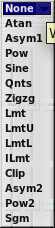
\includegraphics[scale=1.0]{bottom-panel/instrument-edit/PAD/harmonic-content-waveshaping-function.jpg}
   \caption{PADsynth Harmonic Content Editor Wave-Shaping Function}
   \label{fig:padsynth_harmonic_content_editor_waveshaping_function}
\end{figure}

   Values: \texttt{None*, Atan, Asym1, Pow, Sine, Qnts, Zigzg, Lmt,
              LmtU, LmtL, ILmt, Clip, Asym2, Pow2, Sgm}

   The type of wave-shaping distortion has much influence on how the
   overtones are being placed. Sometimes, one gets a "fat" bass, and
   sometimes, high frequencies are added, making the sound "crystal clear".

   \textbf{Atan \& Sigmoid}.
   This is the default setting. It is an easy way to apply loudness to a wave
   without getting undesired high overtones. Thus, it can be used both for
   making instruments that sound like "real" ones, but also for electronic
   music. The transformation turns, roughly said, every amplitude into a
   square amplitude. Thus, sine, power, pulse and triangle turn into a usual
   square wave, while a saw turns into a phased square wave. A chirp wave
   turns into a kind of phase modulated square wave.

   \textbf{Quants} ("Qnts")
   Quantization adds high overtones early. It can be seen as an unnatural
   effect, which is often used for electronic music.  The transformation is a
   bit similar to building the lower sum of a wave, mathematically said. This
   means that the transformation effect turns an "endless high" sampled
   wave into only a few samples. The more distortion one applies, the fewer
   samples will be used. Indeed, this is equivalent to say that more input
   amplification is used. To see this, here is a small sample of code, where
   "ws" is the (correctly scaled amount of input amplification, and "n" the
   number of original samples.

   If one turns on quantisation very high, one might be confused that,
   especially high notes, make no sound. The reason: High frequencies are
   "forgotten" if one samples with only few samples. Also, the sign of an
   amplitude can be forgotten. This behaviour might make some quantisations a
   bit unexpected.

   \textbf{Limiting} ("Lmt*" and "Clip")
   Limiting usually means that for a signal, the amplitude is modified
   because it exceeds its maximum value. Overdrive, as often used for
   guitars, is often achieved by limiting: It happens because an amplifier
   "overdrives" the maximum amplitude it can deliver.

   ZynAddSubFX has two types of limiting. Soft limiting, here as Lmt, means
   that the sound may not exceed a certain value. If the amplitude does so,
   it will simply be reduced to the limiting value. The overtones are
   generated in the lower frequencies first.

   Hard limiting, is also called clipping and abbreviated Clip. This means
   that if the maximum is exceeded, instead of being constant at the limiting
   value, the original signal still has some influence on the output signal.
   Still, it does not exceed the limiting value. For ZynAddSubFX, a signal
   exceeding the limiting value will continue to grow "in the negative". This
   leads to overtones being generated on the full frequency band.

   \itempar{Wsh Wheel}{padsynth!harm editor wsh wheel}
   Harmonic Editor Wave-shaping Wheel?

   \itempar{Filter}{padsynth!harm editor filter}
   Harmonic Editor Filter.
   Sets the type of the harmonic filter.

\begin{figure}[H]
   \centering 
   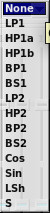
\includegraphics[scale=1.0]{bottom-panel/instrument-edit/PAD/harmonic-content-filter.jpg}
   \caption{PADsynth Harmonic Content Filter}
   \label{fig:}
\end{figure}

   Values: \texttt{None*, LP1, HP1a, HP1b, BP1, BS1, LP2, HP2, BP2,
              BS2, Cos, Sin, LSh, S}

   \itempar{Filter Wheel 1}{padsynth!harm editor filter wheel}
   Harmonic Editor Filter, Wheel 1.

   \itempar{Filter Wheel 2}{padsynth!harm editor filter wheel}
   Harmonic Editor Filter, Wheel 2.
   The knob in the right sets the filter parameter (frequency).

   \itempar{Filter p}{padsynth!harm editor filter p}
   Harmonic Editor Filter, p?

   \itempar{Mod.}{padsynth!harm editor mod}
   Harmonic Editor Modulation.

\begin{figure}[H]
   \centering 
   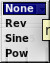
\includegraphics[scale=1.0]{bottom-panel/instrument-edit/PAD/harmonic-content-modulation.jpg}
   \caption{PADsynth Harmonic Content Editor Modulation}
   \label{fig:padsynth_harmonic_content_editor_modulation}
\end{figure}

   Values: \texttt{None*, Rev, Sine, Pow}

   \itempar{Mod. Wheel 1}{padsynth!harm editor mod wheel}
   Harmonic Editor Modulation Wheel 1?

   \itempar{Mod. Wheel 2}{padsynth!harm editor mod wheel}
   Harmonic Editor Modulation Wheel 2?

   \itempar{Mod. Wheel 3}{padsynth!harm editor mod wheel}
   Harmonic Editor Modulation Wheel 3?

   \itempar{Sp.adj.}{padsynth!harm editor spadj}
   Harmonic Editor Spectrum Adjust.
   Adjust the spectrum of the waveform.

   RMS normalize. Enables the RMS normalization method (recommended); this
   keeps the same loudness regardless the harmonic content.

   Below are the harmonics and their phases. One can use them to add to
   oscillator harmonics that has the waveform of the base function.
   Increasing the number of harmonics has virtually no effect on CPU usage. 
   Right click to set a harmonic/phase to the default value. 

\begin{figure}[H]
   \centering 
   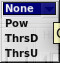
\includegraphics[scale=1.0]{bottom-panel/instrument-edit/PAD/harmonic-content-osc-spectrum-adjust.jpg}
   \caption{PADsynth Harmonic Content Editor Spectrum Adjust}
   \label{fig:padsynth_harmonic_content_editor_spectrum_adjust}
\end{figure}

   Values: \texttt{None*, Pow, ThrsD, ThrsU}

   \itempar{Sp.adj. Wheel}{padsynth!harm editor spadj wheel}
   Harmonic Editor Spectrum Adjust Wheel?

\paragraph{PADsynth / Harmonic Structure / Change / Harmonic}
\label{paragraph:padsynth_harmonic_structure_change_harmonic}

   \begin{enumber}
      \item \textbf{Harmonics Amplitude}
      \item \textbf{Harmonics Bandwidth}
      \item \textbf{Harmonics Scrollbar}
      \item \textbf{Harmonic Shift}
      \item \textbf{Harmonic Shift R} (dialog?)
      \item \textbf{Harmonic Shift preH}
      \item \textbf{Adpt.Harm.}
      \item \textbf{Adpt.Harm. Slider}
      \item \textbf{Adpt.Harm. baseF}
      \item \textbf{Adpt.Harm. pow}
      \item \textbf{Clear}
      \item \textbf{Sine}
      \item \textbf{C}
      \item \textbf{P}
      \item \textbf{Close}
   \end{enumber}

   \itempar{Harmonics Amplitude}{padsynth!harmonics amplitude}
   Harmonics Amplitude.
   Provides 128? sliders for the amplitude of harmonics.

   \itempar{Harmonics Bandwidth}{padsynth!harmonics bandwidth}
   Harmonics Bandwidth.
   Provides 128? sliders for the bandwidth of harmonics.

   \itempar{Harmonics Scrollbar}{padsynth!harmonics scrollbar}
   Harmonics Scrollbar.

   \itempar{Harmonic Shift}{padsynth!harmonics shift}
   Harmonics Shift.

   Values: \texttt{-x to 0 to x?}

   \itempar{Harmonic Shift R}{padsynth!harmonics shift r}
   Harmonics Shift R?.

   \itempar{Harmonic Shift preH}{padsynth!harmonics shift preh}
   Harmonics Shift preH?
   preF in Zyn?

   preF. Set the order of doing the filter and wave-shaper (uncheck to filter
   after wave-shaping, check to wave-shape after filtering).

   \itempar{Adpt.Harm.}{padsynth!harmonics}
   Adaptive Harmonics?

\begin{figure}[H]
   \centering 
   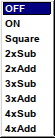
\includegraphics[scale=1.0]{bottom-panel/instrument-edit/PAD/harmonic-content-adaptive-harmonic-type.jpg}
   \caption{PADsynth Adaptive Harmonic Type}
   \label{fig:padsynth_adaptive_harmonic_type}
\end{figure}

   Values: \texttt{OFF*, ON, Square, 2xSub, 2xAdd, 3xSub, 3xAdd, 4xSub, 4xAdd}

   \itempar{Adpt.Harm. Slider}{padsynth!harmonics slider}
   Adaptive Harmonics Slider?

   \itempar{Adpt.Harm. baseF}{padsynth!harmonics basef}
   Adaptive Harmonics Base Frequency?

   \itempar{Adpt.Harm. pow}{padsynth!harmonics pow}
   Adaptive Harmonics Power?

   \itempar{Clear}{padsynth!harmonics clear}
   Harmonics Clear.
   Clears the harmonics settings.

   \itempar{Sine}{padsynth!harmonics sine}
   Harmonics Sine.  
   The user is prompted to "Convert to sine?"
   This seems to reset everything to the state where it has not been
   modified, but that's not certain.

   \itempar{C}{padsynth!harmonics copy}
   Harmonics Copy.

   \itempar{P}{padsynth!harmonics paste}
   Harmonics Paste.

   \itempar{Close}{padsynth!harmonics close}
   Harmonics Close.

\subsection{PADsynth / Envelopes and LFOs}
\label{subsec:padsynth_envelopes_lfos}

\begin{figure}[H]
   \centering 
   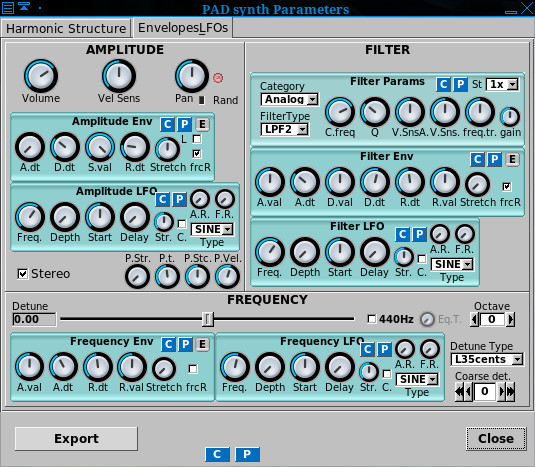
\includegraphics[scale=1.0]{bottom-panel/instrument-edit/PAD/PADsynth-parameters-envelopes-LFOs.jpg}
   \caption{PADSynth Parameters, Envelopes and LFOs}
   \label{fig:padsynth_parameters_envelopes_and_lfos}
\end{figure}

   \begin{enumber}
      \item \textbf{AMPLITUDE}
      \item \textbf{FILTER} (section)
      \item \textbf{FREQUENCY} (section)
      \item \textbf{Export}
      \item \textbf{C}
      \item \textbf{P}
      \item \textbf{Close}
   \end{enumber}

   \itempar{AMPLITUDE}{padsynth!amplitude section}
   See \sectionref{subsec:addsynth_amplitude}.
   This stock dialog section provide volume, velocity sensing, panning, an
   amplitude envelope sub-panel, and an amplitude LFO sub-panel.

   \itempar{FILTER}{padsynth!amplitude section}
   See \sectionref{subsec:addsynth_filter}.

   \itempar{FREQUENCY}{padsynth!amplitude section}
   See \sectionref{subsec:addsynth_frequency}.

   \itempar{Export}{padsynth!export}
   Very similar to 
   \figureref{fig:harmonics_structure_export_dialog}.

   \itempar{C}{padsynth!copy}
   The stock copy dialog.

   \itempar{P}{padsynth!paste}
   The stock paste dialog.

   \itempar{Close}{padsynth!close}
   Close.

%-------------------------------------------------------------------------------
% vim: ts=3 sw=3 et ft=tex
%-------------------------------------------------------------------------------
